\documentclass[tikz,border=0pt]{standalone}
\usepackage[american]{circuitikz}
\usetikzlibrary{arrows.meta,calc,positioning,decorations.pathmorphing,patterns}
\definecolor{zyloTeal}{HTML}{174A5B}
\definecolor{zyloTealTwo}{HTML}{246B7A}
\definecolor{zyloInk}{HTML}{1F2933}
\definecolor{zyloSoft}{HTML}{EAF4F4}
\definecolor{zyloPaper}{HTML}{F8FAFB}
\definecolor{zyloLine}{HTML}{44606B}
\definecolor{zyloOrange}{HTML}{D97706}
\begin{document}
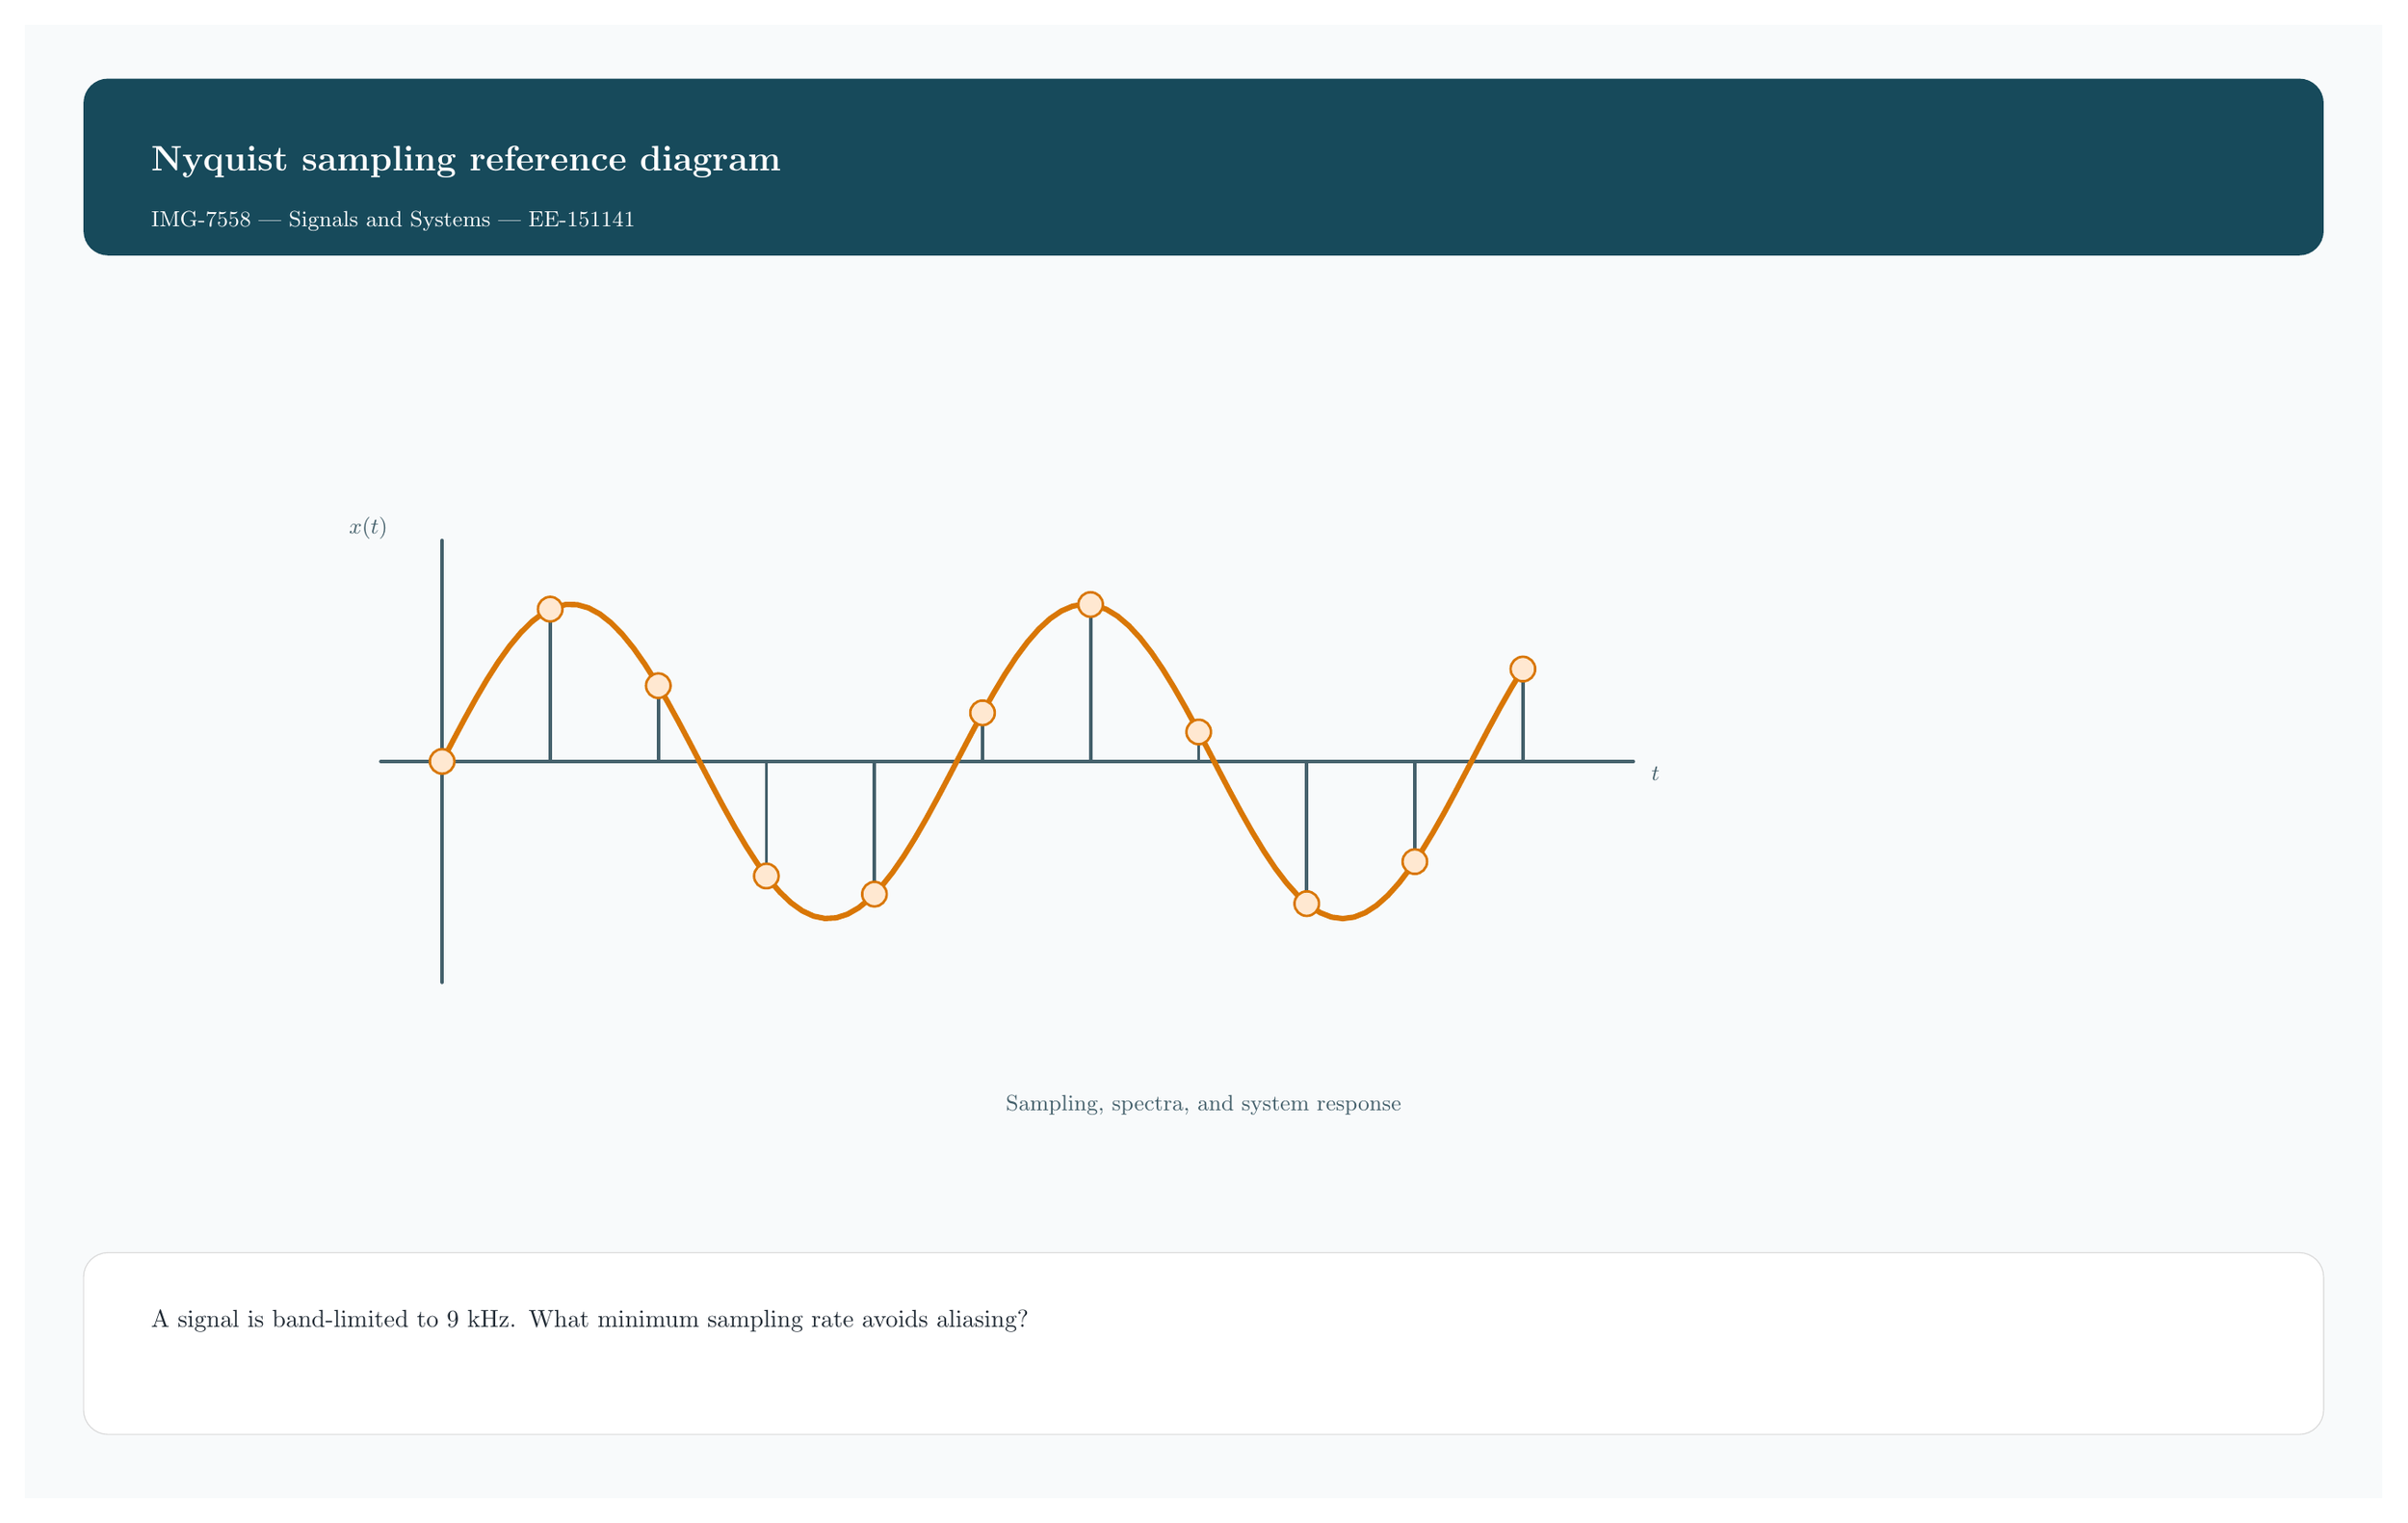
\begin{tikzpicture}[x=1pt,y=-1pt,>=Latex,line cap=round,line join=round]
\path[fill=zyloPaper] (0,0) rectangle (960,600);
\path[fill=zyloTeal,rounded corners=10pt] (24,22) rectangle (936,94);
\node[anchor=west,text=white,font=\bfseries\Large] at (48,56) {Nyquist sampling reference diagram};
\node[anchor=west,text=white!82,font=\small] at (48,80) {IMG-7558 | Signals and Systems | EE-151141};
\tikzset{wire/.style={draw=zyloTeal,line width=2.2pt},thinwire/.style={draw=zyloLine,line width=1.35pt},accent/.style={draw=zyloOrange,line width=2.2pt},box/.style={draw=zyloTealTwo,fill=zyloSoft,line width=1.5pt,rounded corners=8pt}}
\draw[thinwire] (145,300) -- (655,300);
\draw[thinwire] (170,210) -- (170,390);
\draw[accent] (170,300) -- (174.583,291.231) -- (179.167,282.628) -- (183.75,274.352) -- (188.333,266.56) -- (192.917,259.399) -- (197.5,253.003) -- (202.083,247.494) -- (206.667,242.976) -- (211.25,239.532) -- (215.833,237.23) -- (220.417,236.111) -- (225,236.197) -- (229.583,237.487) -- (234.167,239.956) -- (238.75,243.557) -- (243.333,248.223) -- (247.917,253.865) -- (252.5,260.378) -- (257.083,267.638) -- (261.667,275.508) -- (266.25,283.841) -- (270.833,292.478) -- (275.417,301.257) -- (280,310.012) -- (284.583,318.578) -- (289.167,326.794) -- (293.75,334.505) -- (298.333,341.565) -- (302.917,347.841) -- (307.5,353.214) -- (312.083,357.584) -- (316.667,360.868) -- (321.25,363.003) -- (325.833,363.951) -- (330.417,363.692) -- (335,362.232) -- (339.583,359.598) -- (344.167,355.84) -- (348.75,351.029) -- (353.333,345.255) -- (357.917,338.628) -- (362.5,331.272) -- (367.083,323.326) -- (371.667,314.941) -- (376.25,306.273) -- (380.833,297.487) -- (385.417,288.749) -- (390,280.223) -- (394.583,272.07) -- (399.167,264.444) -- (403.75,257.488) -- (408.333,251.334) -- (412.917,246.098) -- (417.5,241.879) -- (422.083,238.756) -- (426.667,236.788) -- (431.25,236.012) -- (435.833,236.444) -- (440.417,238.074) -- (445,240.872) -- (449.583,244.785) -- (454.167,249.74) -- (458.75,255.642) -- (463.333,262.382) -- (467.917,269.831) -- (472.5,277.849) -- (477.083,286.284) -- (481.667,294.979) -- (486.25,303.768) -- (490.833,312.486) -- (495.417,320.968) -- (500,329.055) -- (504.583,336.594) -- (509.167,343.443) -- (513.75,349.473) -- (518.333,354.569) -- (522.917,358.636) -- (527.5,361.597) -- (532.083,363.396) -- (536.667,364) -- (541.25,363.396) -- (545.833,361.597) -- (550.417,358.636) -- (555,354.569) -- (559.583,349.473) -- (564.167,343.443) -- (568.75,336.594) -- (573.333,329.055) -- (577.917,320.968) -- (582.5,312.486) -- (587.083,303.768) -- (591.667,294.979) -- (596.25,286.284) -- (600.833,277.849) -- (605.417,269.831) -- (610,262.382);
\draw[thinwire] (170,300) -- (170,300); \draw[draw=zyloOrange,fill=orange!18,line width=1pt] (170,300) circle (5);
\draw[thinwire] (214,300) -- (214,238.011); \draw[draw=zyloOrange,fill=orange!18,line width=1pt] (214,238.011) circle (5);
\draw[thinwire] (258,300) -- (258,269.168); \draw[draw=zyloOrange,fill=orange!18,line width=1pt] (258,269.168) circle (5);
\draw[thinwire] (302,300) -- (302,346.654); \draw[draw=zyloOrange,fill=orange!18,line width=1pt] (302,346.654) circle (5);
\draw[thinwire] (346,300) -- (346,354.037); \draw[draw=zyloOrange,fill=orange!18,line width=1pt] (346,354.037) circle (5);
\draw[thinwire] (390,300) -- (390,280.223); \draw[draw=zyloOrange,fill=orange!18,line width=1pt] (390,280.223) circle (5);
\draw[thinwire] (434,300) -- (434,236.126); \draw[draw=zyloOrange,fill=orange!18,line width=1pt] (434,236.126) circle (5);
\draw[thinwire] (478,300) -- (478,288.008); \draw[draw=zyloOrange,fill=orange!18,line width=1pt] (478,288.008) circle (5);
\draw[thinwire] (522,300) -- (522,357.909); \draw[draw=zyloOrange,fill=orange!18,line width=1pt] (522,357.909) circle (5);
\draw[thinwire] (566,300) -- (566,340.795); \draw[draw=zyloOrange,fill=orange!18,line width=1pt] (566,340.795) circle (5);
\draw[thinwire] (610,300) -- (610,262.382); \draw[draw=zyloOrange,fill=orange!18,line width=1pt] (610,262.382) circle (5);
\node[font=\small,text=zyloLine] at (664,305) {$t$}; \node[font=\small,text=zyloLine] at (140,205) {$x(t)$};
\node[font=\small,text=zyloLine] at (480,440) {Sampling, spectra, and system response};
\path[draw=black!15,fill=white,rounded corners=10pt] (24,500) rectangle (936,574);
\node[anchor=west,text width=860pt,align=left,text=zyloInk,font=\normalsize] at (48,528) {A signal is band-limited to 9 kHz. What minimum sampling rate avoids aliasing?};
\end{tikzpicture}
\end{document}
